% Artyom Voronin
%     _                     
% ___| |__  _ __  _ __ ___  
%/ __| '_ \| '_ \| '_ ` _ \ 
%\__ \ |_) | |_) | | | | | |
%|___/_.__/| .__/|_| |_| |_|
%          |_|              
%
% Brno, 2021


% ----------------------------------------------------------------------------- 

% ----------------------------------------------------------------------------- 

\chapter{Signal-Based PdM}
This chapter introduces the signal-based method applied to a measured
dataset.  The whole solution procedure will be presented on the example of
the development solution on the flow sensor \ref{sec:flow_example}.  Most
of the methods used in this chapter are closely related between FDI and PdM
approaches. These methods work directly with the measured signal by
extracting condition indicators and training the classification model. It
is possible to do fault detection and classification using this model.


\section{FDI methods}\label{sec:easy_fdi}
There are simple solutions that offer themselves. For example, the
proximity sensor can be used to monitoring whether the actuator has reached
the position in the expected interval or not. Based on these data, it can
be concluded whether the device performs its function or a fault has
occurred.  Similarly, we can monitor the flow course, and if this course
exceeds any given threshold, then a fault has occurred.  Using more complex
methods, we can not only show the occurrence of faults but also classify
the cause. The implementation of these algorithms will be further discussed
in this chapter.

\section{Data Management and Preprocessing}
Before the final solution was developed in the whole dataset, the smaller
dataset was used for experiments and planning algorithms. 

\subsection{Data Storage}
\paragraph{Manage Data}

First, a folder structure was created to collect all measured and
calculated data. The measured signals were given in 6 large files with a
".mat" extension and divided into smaller files with only one measurement
each.  Data files have been reshaped to Data Ensembles \cite{} format used
for Condition monitoring purposes. This format allows processing data
without copying the whole dataset to memory at once but processes them one
by one. In large datasets it gives an option to manipulate with data
without problems with allocated memory.  The full dataset contains 4840
measurements. Each measurement includes a 10-second recording of all
signals collected from moving the piston up and down.

\paragraph{Labels}
The whole dataset was divided into 20 Labels by place of fault accumulate: 
\begin{itemize}
    \item Healthy
    \item Throttle valve 1
    \item Throttle valve 2 
    \item Small damper bottom
    \item Small damper upper
    \item Large dampers 
    \item And combinations of these faults
\end{itemize}

\subsection{Data Exploration}
Data from each of the eight sensors \ref{tab:sensors_tab} were explored in an attempt to find
measurement errors or anomalies in data.  Figure \ref{fig:flow_sig} shown
an example of the flow signal in different operation conditions. 

\begin{figure}[h!]
    \centering
    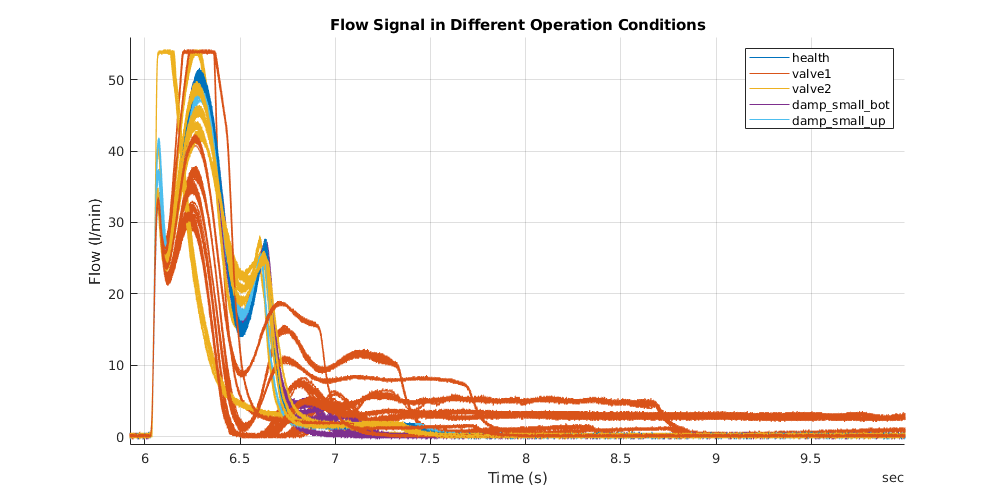
\includegraphics[width=1\textwidth]{sb_flow_signal.png}
    \caption{Flow Signal in Different Operation Conditions}
    \label{fig:flow_sig}
\end{figure}


%There are eight types of sensors:
%\begin{enumerate}
%    \item Linear encoder
%    \item Flow sensor
%    \item Pressure sensor
%    \item Temperature sensor
%    \item Accelerometer
%    \item Strain gauge
%    \item Microphones
%    \item Proximity sensors
%\end{enumerate}

\subsection{Preprocessing}

After the data has been processed and organized in one datastore, the
possibility arises to perform signal preprocessing.  Preprocessing includes
smoothing, filtering, detrend the signal, and missing value removal.

The datastore contains some signals, such as an encoder, that is very
accurate. There is no preprocessing needed to apply. Signals noisier
(pressure signal or strain) have to be preprocessed and applied algorithms
to noise reduction such as smoothing and filtering concerning the
preservation of the information base. However, during experiments turned
out that non preprocessed signals have better performance. For example, the
preprocessed pressure classification model gives 78 \% accuracy; model
trained on CI from the raw pressure signal offers approximately 82 \%.

\section{SB Methods and Flow Sensor as an Example}\label{sec:flow_example}
In this section, signal-based methods were applying to the flow sensor as a
case study example.  The rest of the sensors was processed in the same way;
however, each required an individual approach.

\subsection{Flow Sensor Data}
There are two flow signals in the datastore. Both are connected to port A
in scheme \ref{}. Signals were sampled in 1kHz frequency; thus, in 10
seconds, there are 10000 points measured. 

\begin{itemize}
    \item Flow Extrusion
    \item Flow Contraction
\end{itemize}

\subsection{Condition Indicators Extraction}

\begin{figure}[h!]
    \centering
    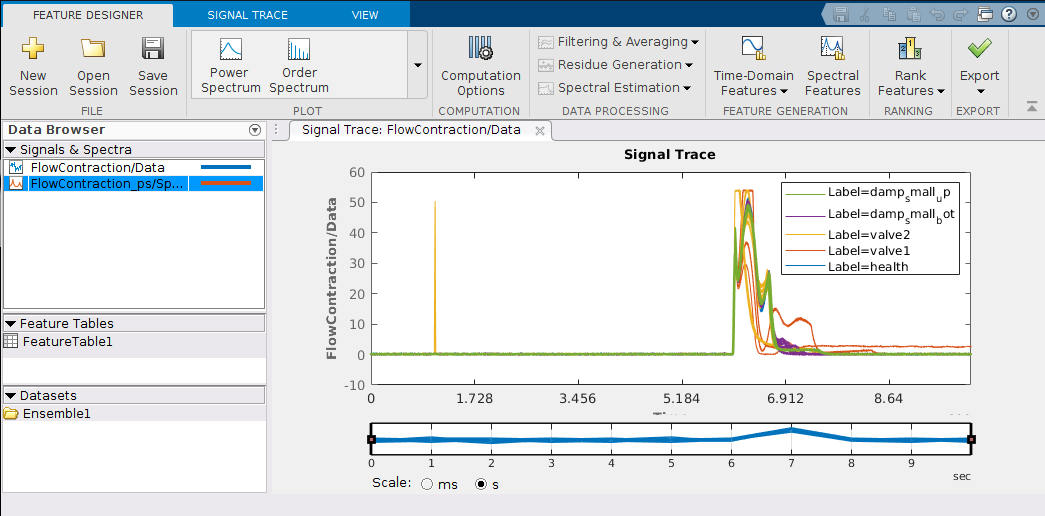
\includegraphics[width=1\textwidth]{dfd_app.png}
    \caption{Diagnostic Features Designer App Interface}
    \label{fig:dfd_app}
\end{figure}

One of the reasons to use Matlab Data Ensemble format to manage the data
instead of others is to use the Diagnostic Feature Designer App
\ref{fig:dfd_app}.
This app provides an intuitive environment for extracting both statistical
condition indicators and power spectral density calculations with the
following extraction of frequency condition indicators. It is also possible
to generate Matlab functions to deploy the algorithms on a bigger scale.

\paragraph{Statistical Condition Indicators}

For every flow signal in the dataset, statistical condition indicators were calculated: 
\begin{itemize}
    \item Mean
    \item Standard deviation
    \item RMS
    \item Peak value
    \item Kurtosis
    \item Clearance factor
    \item Crest factor
    \item Impulse factor
    \item etc.
\end{itemize}


\paragraph{Frequency Domain Condition Indicators}

\begin{figure}[h!]
    \centering
    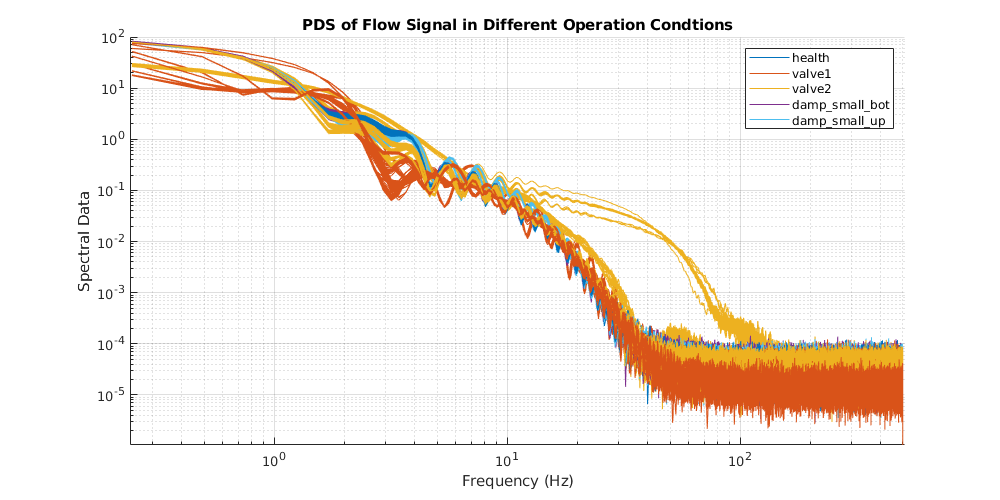
\includegraphics[width=1\textwidth]{sb_flow_spec.png}
    \caption{Welch's Power Spectral Density of the Flow Signal}
    \label{fig:flow_sp}
\end{figure}


Using Welch's power spectral density estimation \ref{fig:flow_sp}, frequency CI were
calculated: 

\begin{itemize}
\item First five peaks amplitude
\item Peaks frequencies
\item Spectrum band power
\end{itemize}


Extracted condition indicators were written to files with signals and
easily acceptable. After each data file contains complete information about
one measurement:
\begin{itemize}
    \item Measured signals
    \item Setting parameters (valves, dampers, load)
    \item Power spectrum calculated from measured signals
    \item Statistical and Frequency features extracted from signals
\end{itemize}

Moreover, a table was created, which contains all condition indicators
extracted, to prepare the train and test dataset for the classification
model.

\subsection{Condition Indicators Ranking}
The table of calculated condition indicators contains 25 statistical and
frequency CI. To train a classification model, it is good practice to
reduce the number of features or transform them with PCA algorithm and use
only first $n$ principal components, to remove linearly dependent condition
indicators.  According to section \ref{} Analysis of Variance (ANOVA),
specifically in our case Kruskal – Wallis one-way ANOVA algorithm was used. 


The result is a sorted table \ref{tab:sorted_ci} of condition indicators depending on
how much variance a particular condition indicator can describe in the
dataset.

\begin{table}[h]
        \centering
    \begin{tabular} {|c|c|c|} \hline
          & Features & Kruskal-Wallis \\ \hline
        1 & FlowContraction\_ps\_spec/PeakAmp1 & 1.4815e+03 \\ \hline
        2 & FlowContraction\_stats/CrestFactor & 967.6028 \\ \hline
        3 & FlowContraction\_ps\_spec/PeakAmp3 & 865.7571 \\ \hline
        4 & FlowContraction\_stats/Mean        & 567.6620 \\ \hline
        5 & FlowContraction\_ps\_spec/PeakAmp4 & 460.0924 \\ \hline
    \end{tabular}
    \caption{First Five Ranked Condition Indicators using ANOVA}
    \label{tab:sorted_ci}
\end{table}

Figure \ref{fig:sb_scatt_mat} shows the scatter plot of the first three condition
indicators for normal behavior and fault condition caused by the change of
throttle valve 1.
The first five condition indicators ranked by the ANOVA algorithm were used
for training the final model on all 20 labels.

\begin{figure}[h!]
    \centering
    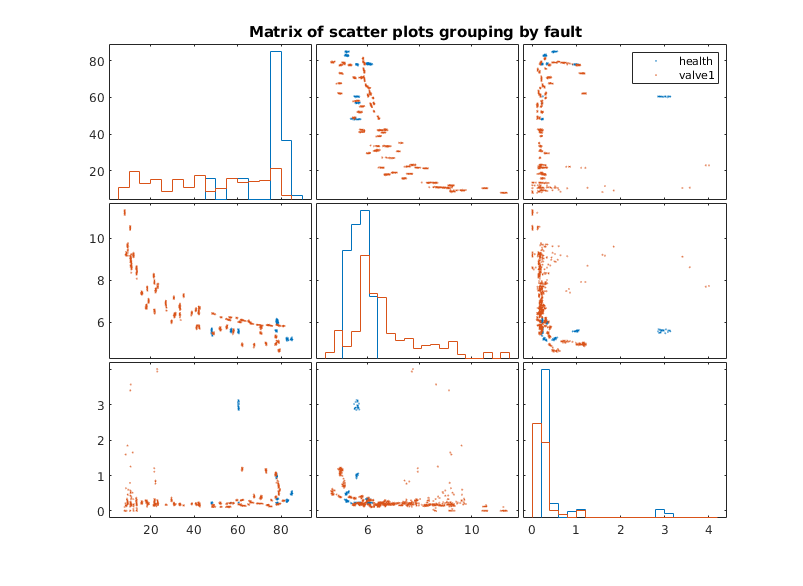
\includegraphics[width=0.8\textwidth]{sb_scatter_matrix.png}
    \caption{Example of Scatter Plot with different CI}
    \label{fig:sb_scatt_mat}
\end{figure}


\subsection{Train Classification Model}
The main goal of the classification task is to train a model that can
predict the fault code or label signalized about pneumatic actuator
behavior by calculated condition indicators.

There are many classification models, but it is best to try different
variants and be satisfied with the best result from a practical point of
view.  The Classification Learner App from the Machine Learning Toolbox
tool can be used for experiments and iterative tuning of different
condition indicators and classification models. It is possible to try
several models, apply the PCA algorithm, interactively draw Scatter plot
and Confusion Matrix, and generate functions for practical applications.

\paragraph{Train, Test Datasets} By splitting data to train and test
datasets, we can ensure that the training model outcomes are valid. The
cross-validation resampling procedure to prevent model overfitting was used
during the model fitting.

\paragraph{Classification Model Performance}


Trained classification models show excellent results on the test dataset
for all three situations: using all CI, after applying the PCA algorithm
and using the first five CIs recommended by the ANOVA algorithm.  The
accuracy evaluations of the models are shown in Table
\ref{tab:classification_perfomance}.

\begin{table}[h!]
    \centering
    \begin{tabular}{|c|c|c|}
        \hline
        \textbf{approach} & \textbf{model}     &  \textbf{accuracy [\%]} \\
        \hline
        all features      &  Bagged Trees      &  99.45  \\
        PCA               &  Bagged Trees      &  95.18  \\
        ANOVA             &  Fine KNN          &  97.52  \\
        \hline
    \end{tabular}
    \caption{All Features vs PCA vs ANOVA perfomance}
    \label{tab:classification_perfomance}
\end{table}

Figure \ref{fig:conf_matrix} shows the confusion matrix from the Fine KNN
classification model by training on data using the ANOVA algorithm.  From
the confusion matrix, it is clear that combined faults in the dataset were
not observed much. However, the model can successfully resolve these fault
conditions too.

\begin{figure}[h!]
    \centering
    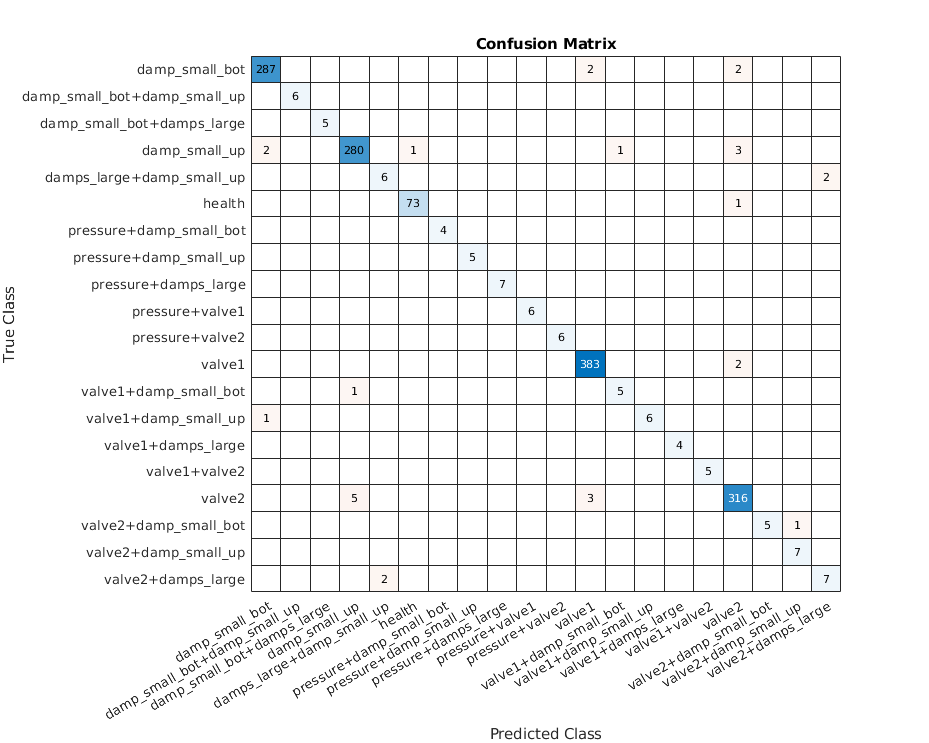
\includegraphics[width=1\textwidth]{sb_confusion_matrix.png}
    \caption{Fine KNN trained on ANOVA Dataset Confusion Matrix}
    \label{fig:conf_matrix}
\end{figure}

From a practical point of view, in this particular case, the use of the
ANOVA algorithm allows not only to reduce the number of CIs for prediction
on the model but also to calculate from the signal, not 25 CIs but only 5. 

Considering this fact, deploy this algorithm on a bigger scale on many
devices, where the calculation complexity plays a role, using the ANOVA
algorithm is justified.

\newpage
\section{Summary All Sensors Comparison}\label{sec:sensors_summary}

Surprisingly, all sensors showed satisfactory results on the measured
dataset.  Processing the entire dataset is a very demanding operation in
terms of calculation. Therefore, only the final solutions were added to the
attachments. The results for all sensors can be verifying by running
matlab-live-script \textit{sb/signal\_based\_live.mlx}.

Table \ref{tab:sensors_final} compares all the sensors used in terms of the
accuracy achieved on the test datasets and the approximate prices of the
sensor itself taken from open sources.  Graph \ref{fig:sensors_final_bar}
visualizes these data. Here are some notes on each of the sensors. 



\begin{table}[h]
    \centering
    \begin{tabular}{|c|c|c|c|c|c|c|c|}
        \hline
        \textbf{Sensor}   & Acc & Encoder & Flow & Mics & Pressure & Proximity & Strain \\
        \hline
        \textbf{Accuracy [\%]} & 91.6 & 96.1 & 97.2 & 95.8 & 76.6 & 80.5 & 95.0 \\
        \hline
        \textbf{Cost [czk]} & 2x 3500 & 25000 & 6000 & 3x 500 & 1000 & 2x 1000 & 15000 \\
        \hline
    \end{tabular}
    \caption{Comparison of sensors from accuracy/cost perspective}
    \label{tab:sensors_final}
\end{table}

\begin{figure}[h!]
    \centering
    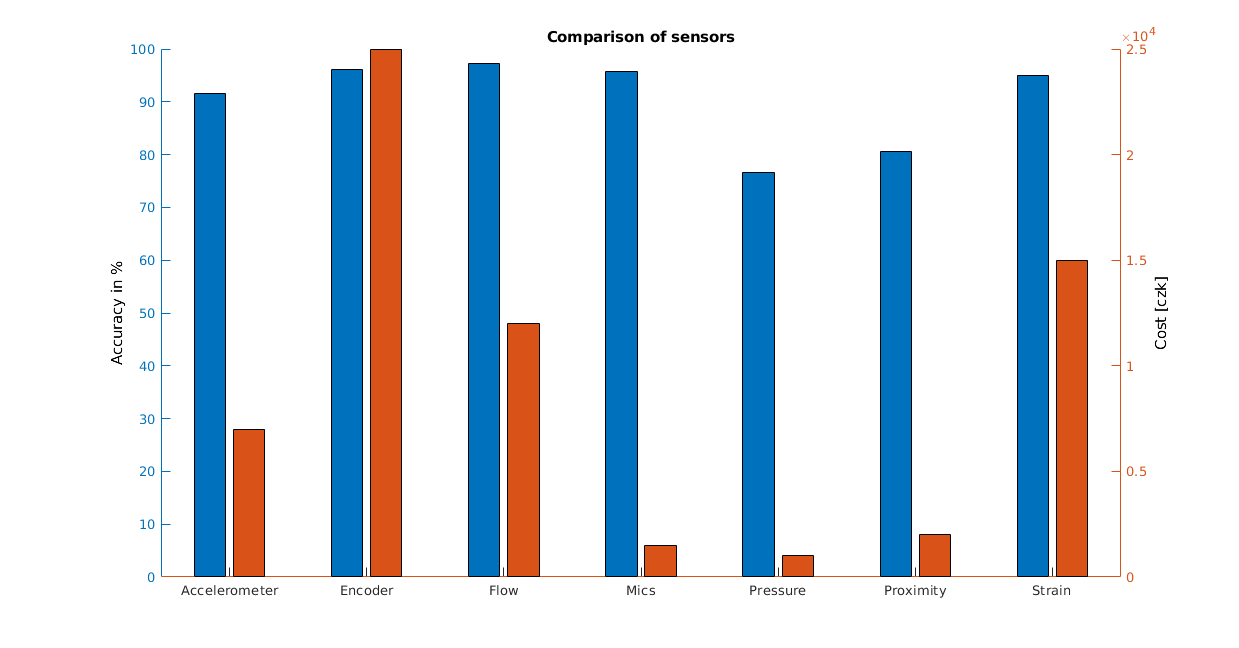
\includegraphics[width=1\textwidth]{sensors_final_bar.png}
    \caption{Comparison of sensors from accuracy/cost perspective}
    \label{fig:sensors_final_bar}
\end{figure}

\subsection{Temperature sensor}
Temperature sensors do only one measurement during the experiment.  These
values can be represented as condition indicators without any
manipulations. Plotting data from the dataset \ref{fig:temp_scatter} shows
that they correlated to an ambient temperature that is different in various
measurement days. These data are sensitive to ambient conditions and
measured data, not representative. The classification model trained on this
data not robust in real life.


\begin{figure}[h!]
    \centering
    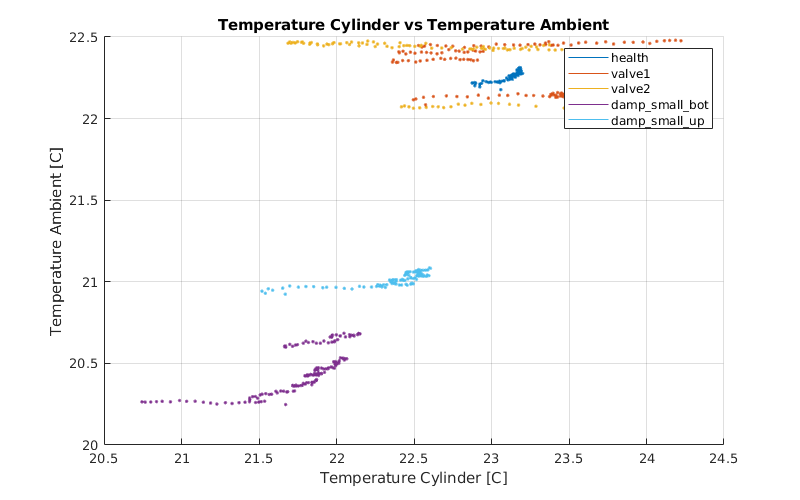
\includegraphics[width=1\textwidth]{sb_temp.png}
    \caption{Scatter plot of temperature measured data}
    \label{fig:temp_scatter}
\end{figure}

\subsection{Encoder}
A linear magnetic encoder is a perfect development sensor-tool for
understanding system behavior and algorithm design. Up to three signals,
displacement, speed, acceleration, can be available from one sensor. The
trained classification model shows perfect results. From a practical point
of view, the financial cost of purchasing, installing, and maintaining the
sensor is unsuitable compared to cheaper sensors with similar prediction
accuracy.

\subsection{Microphones}
Cheap, good results, but maybe problems with real life integration (noise
from another machines). Another problem cannot be modeled in simulation
system. For predictive purposes require data from real model.


\subsection{Accelerometers}
There are two accelerometer sensors. Each sensor contains two signals on
the x, y-axis.  One sensor is placed on the movable part of the stand
device; the second is on the statical part without movement and measure
only vibrations. Sensors show good accuracy; choosing one of the two
accelerometers, the static one, is preferable.

\subsection{Proximity Sensors}
As mentioned before, proximity sensors can be used for simple inspection
purposes \ref{sec:easy_fdi}. Proximity sensors are digital and provide only
statistical condition indicators; from statistical CI offers valuable
information, only a few CI's due to signal shape.

\subsection{Flow Sensors}
Flow sensors achieve the best results. It is possible to achieve $\approx$ 97
\% accuracy using only one sensor. If the practical application requires
maximum accuracy, the flow sensor is the best candidate. Nothing less in
terms of price is an expensive sensor.

\subsection{Air Pressure}
The pressure sensor measures the pressure in the reservoir. Data from this
sensor is not fully informative for the possibilities of predicting and
identifying a fault condition. This sensor showed low accuracy compared to
the others. From an economic view, combining a pressure sensor with another
sensor does not make sense due to existing sensors such as microphones that
are better from an accuracy/cost perspective.

\subsection{Strain Gauge}
Strain Gauge showed excellent results, but in general, it is similar to an
encoder because it is an expensive sensor that requires maintenance.  From
a practical point of view, there are better candidates for industrial
applications.
